\documentclass[10pt,conference,compsocconf]{IEEEtran}

\usepackage{hyperref}
\usepackage{graphicx}	% For figure environment
\usepackage{tabu}

\begin{document}

\title{CS-433 - Machine Learning - Project 1}

\author{
  Eliott Joulot, Jelena Banjac, Kevin Pelletier\\
  \textit{Department of Computer Science, EPFL Lausanne, Switzerland}
}

\maketitle

\begin{abstract}
This report concerns project 1 of the Machine Learning course (CS-433) at EPFL. It consists in using Machine Learning algorithms on datasets provided by the CERN, with the aim of classifying events measured by the ATLAS experiment, distinguishing events originating in the Higgs boson decay signature.
\end{abstract}


\section{\textbf{Introduction} }

The Higgs boson is an elementary particle in the Standard Model [1], which provides an explanation on why other particles have mass. During a collision at high speeds, protons generate smaller particles as by-products of the collision, and at times these collisions produce a Higgs boson. As Higgs boson [2] decays rapidly into other particles, scientists don't observe it directly, but rather measure its decay signature. 

Many decay signatures look similar, and in this project we used different machine learning algorithms to train models for predicting whether the given event's signature was the result of a Higgs boson (signal) or some other process/particle (background) [3].

An important part in the training of the models is the preprocessing and feature selection from the dataset. Separation of entries by relevant features, dealing with missing values, and setting hyperparameters proved to be crucial to achieve a high accuracy level.

In chapter II we will describe what how and why we cleaned the data, as well as the ways we used to train our models. In chapter III we discuss implemented machine learning models together with the performance analysis. In chapter IV we display our final results and kaggle score. Finally, we summarize our work in chapter V.



\section{\textbf{Data \& preprocessing}}

In this section we wil describe how we first explored the data and performed a preprocessing and cleaning. The following subsections will shortly describe what were our observations and actions we performed towards preparing data for running a different models. In addition, a more detailed report can be found in Jupyter Noteboos we used to interactively execute our code.

\subsection{Data exploration}

We were given two sets of data in \textit{csv} format, a training and a test set. They are signal samples of $30$ different features. In the training set, an additionnal output column $y_n$ is provided with a value depending on whether the recorded signal corresponds to an actual event ($1$) or to background noise ($-1$).

\subsection{Preprocessing}

After exploring closely all the data we have, we found that only a quarter of the dataset is actually complete. Indeed, $11$ features out of the $30$ have missing values (encoded as $-999$). However, we found that they are closely linked to the $jet$ property. Thus, we took the approach of separating the data based on this property, and applying Machine Learning algoritms to compute the most likely value for each missing one, using the correct data we have.

The first step was then to separate our data into 4, according to the $jet$ number. The incorrect values were then extracted from the obtained data to create 4 training datasets. On each of them, we were able to apply models that will allow us to make predictions on missing values using ridge regression and data augmentation. In order to obtain a more accurate result, we have carefully adapted the model for all 4 $jet$ numbers. Indeed, we realized for example that a degree $2$ for polynomial expansion of $jet0$ features was more effective, whereas it brought too much overfitting to the others.

This approach gave us some very good results, and we managed to get a good model by tuning hyperparameters.

\begin{figure}[h]
  \centering
  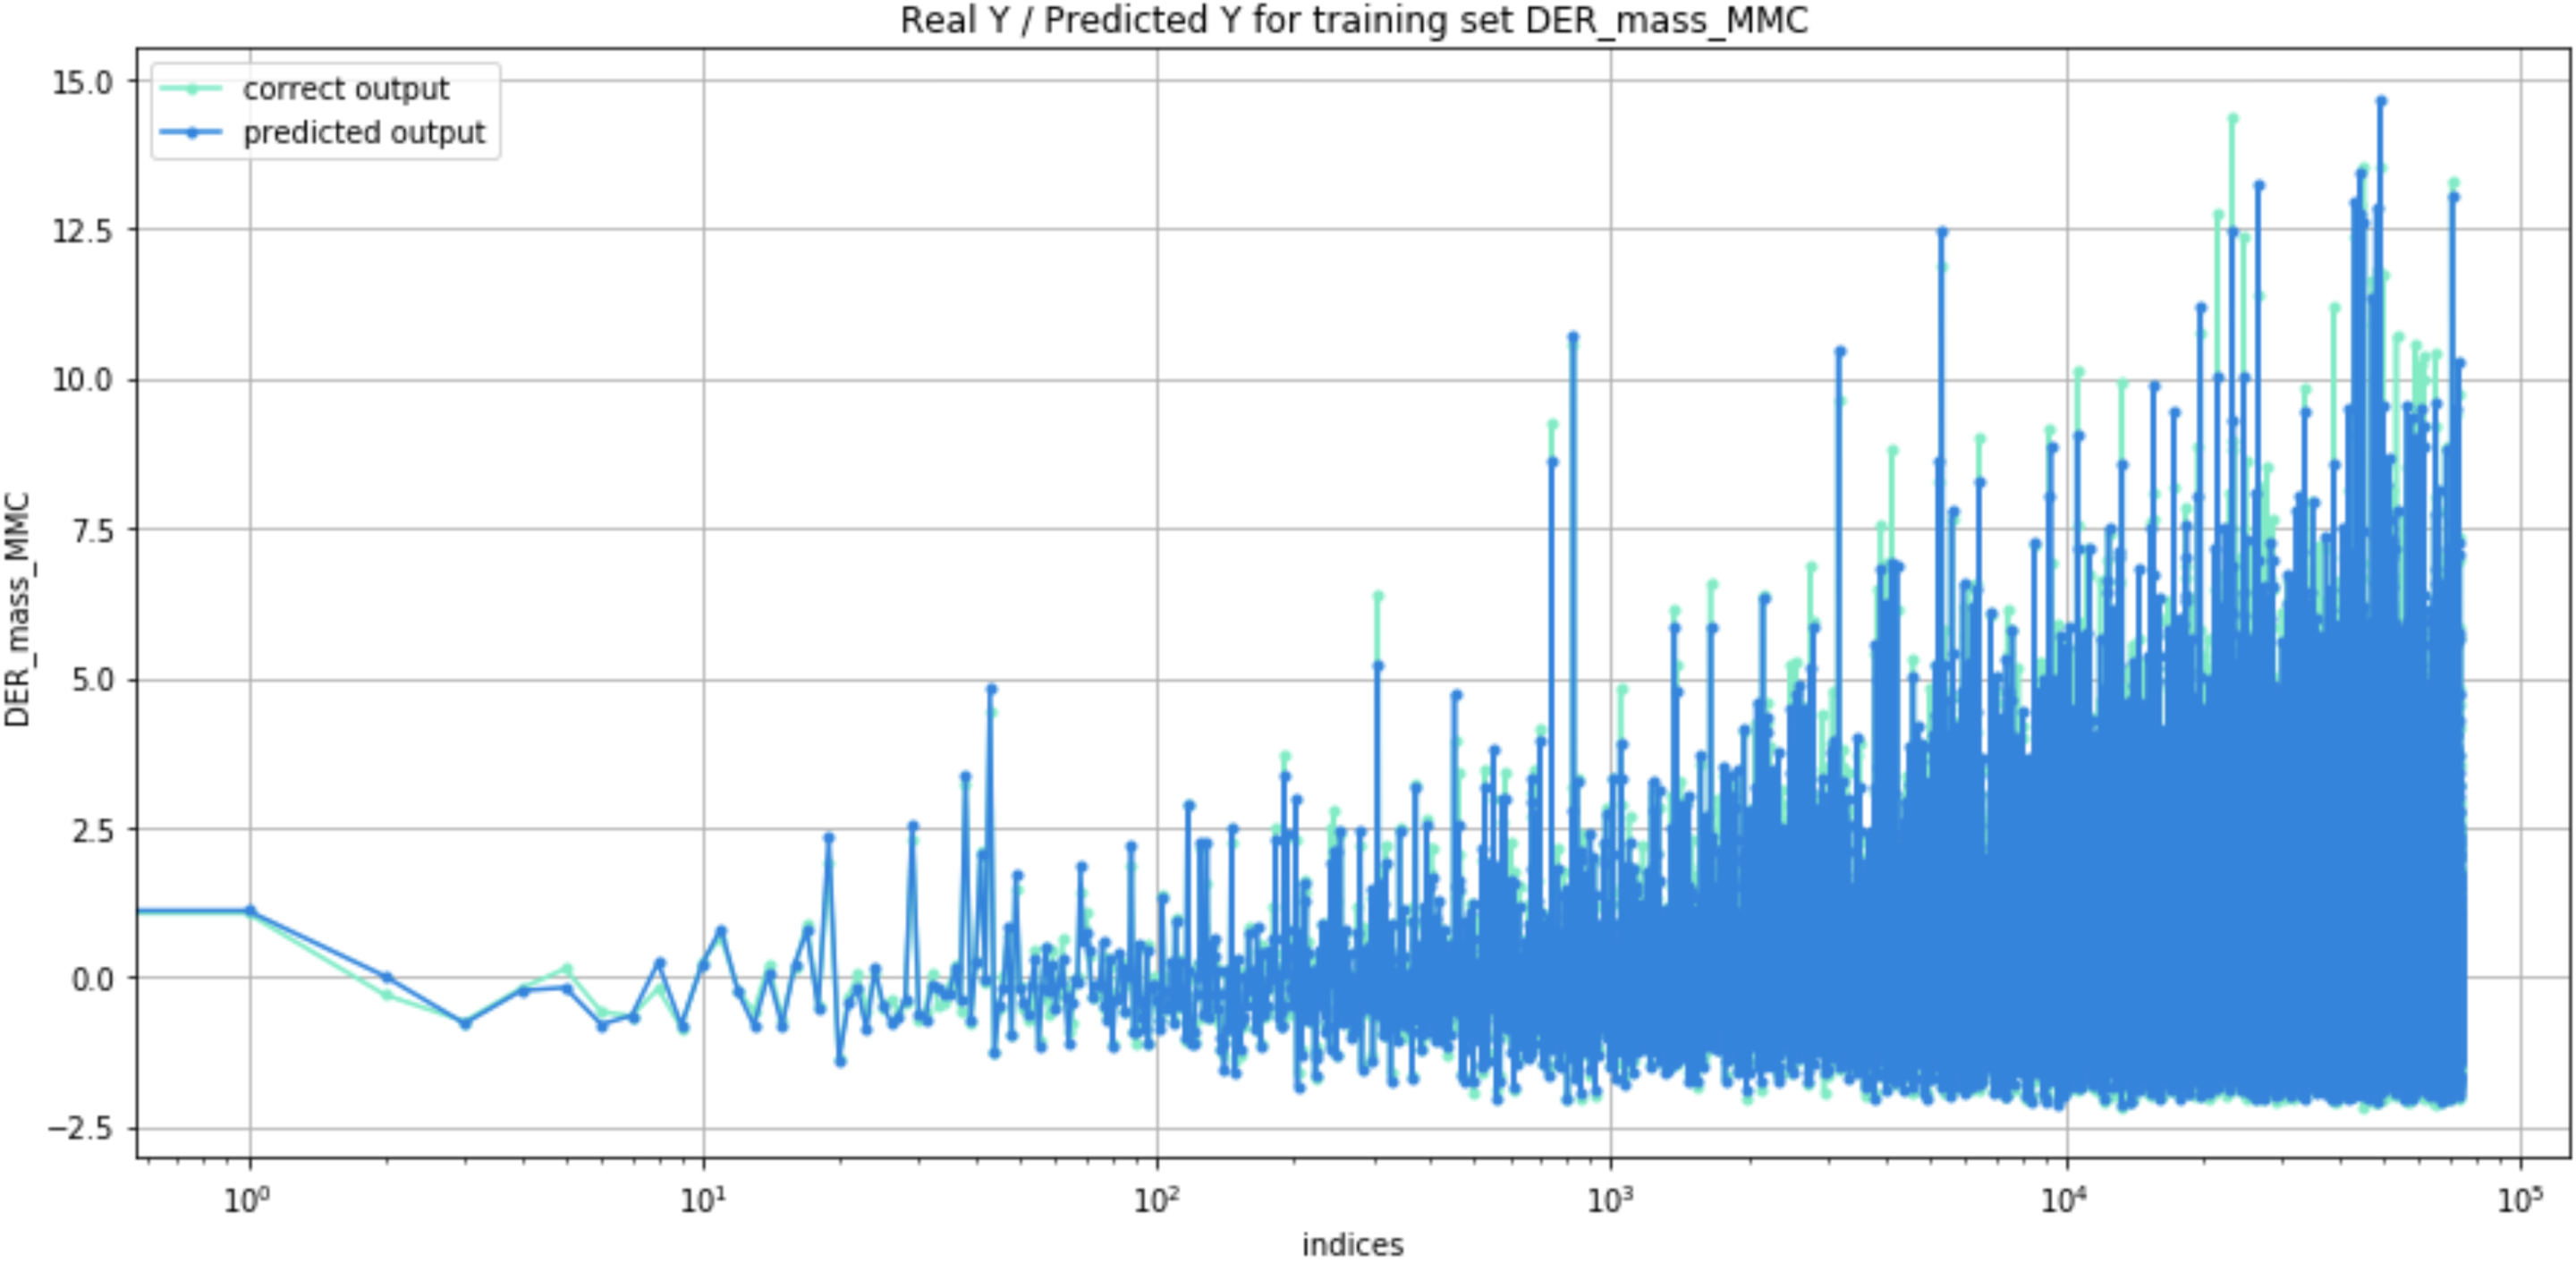
\includegraphics[width=1\columnwidth]{cleaning_model}
  \caption{Prediction accuracy on training values.}
\end{figure}

Using our models, we were therefore able to replace all the missing values in our 4 datasets. 

Of course, all the data wrangling which we performed on the train set, was also done on the test set.

\section{\textbf{Machine learning models}}

In the following subsections, the outcomes of performance of machine learning models from exercises will be discussed.  

The models were tested on the provided training dataset that was split in training and test subdatasets in order to measure the performance of models.

\subsection{Model Selection}

The following models were tested:
\begin{itemize}
  \item Gradient and stochastic gradient descent
  \item Least squares
  \item Ridge regression, with polynom basis
  \item Logistic and regularized logistic regression
\end{itemize}\vspace*{10px}

\begin{tabu} to 0.46\textwidth { | c | X[c] | X[c] | }
  \hline
  Model & Accuracy & Loss \\ 
  \hline 
  Least squares & 74.18\% & 0.8237 \\ 
  Least squares GD & 62.81\% & 0.7582 \\ 
  Least squares SGD & - & 0.7582 \\ 
  Ridge Regression & 74.14\% & 0.3392 \\ 
  Logistic regression & 72.23\% & - \\ 
  \hline
\end{tabu}\vspace*{10px}

The table above summarizes our results for all models. Considering tem, the ridge regression model was selected for submission.

\subsection{Data Expansion}

Before fitting the model, we have done a polynomial expansion of the features in our train and test sets to let the model learn more complex dependencies, adding:
\begin{itemize}
  \item $x_n^k$, with $k \in \{1, ..., d\}$. The optimal value of $d$ was determined with grid search for each subset of data.
  \item Cross term products: $x_i \times x_j, \forall i,j \in \{1, ..., D=30\}$. To extract correlation between pairs of features.
  \item Cross term squared products: $x_i^2 \times x_j^2, \forall i,j \in \{1, ..., D=30\}$.
\end{itemize}

\subsection{Cross Validation}

We perform 10-fold cross validation in order to improve the reliability of the model. It consists in splitting the training data set into 10 subsets of equivalent size. 9 subsets are then used to train the models, and the last one to test them. This process is repeated for all 10 combinations of training and testing subsets possible. It allows us to make sure a model is stable and that we did not overfit our model on the training set.

\begin{table}
\centering
\begin{tabu} to 0.4\textwidth { | X[c] | X[c] | X[c] | }
  \hline
  Model & $d$ & $\lambda$ \\ 
  \hline 
  0 & 7 & $1.10^{-4}$ \\ 
  1 & 8 & $1.10^{-4}$ \\ 
  2 & 8 & $1.10^{-4}$ \\ 
  3 & 8 & $1.10^{-4}$ \\ 
  \hline
\end{tabu}
\caption{Optimal parameters selected for each model}
\label{table:table1}
\end{table}
 
\subsection{Parameters Definition}

We finally used grid search to set the values of the different hyperparameters that we would use in our model. We did that for the four subsets of data (jet number) we have. The results are shown in \ref{table:table1}.


\section{\textbf{Results}}

Once we finished expanding the data and setting the hyperparameters, we were able to do the final submission on the test data, and save the predicted labels for the kaggle submission. The final score obtained on kaggle was \textbf{81.883\%}.

\section{\textbf{Summary}}

The aim of our project was to build a highly accurate machine learning model for categorizing proton collision events. In our work, we explored four different implementations of the linear regression algorithm and two additional algorithms for the logistic regression. Our research included preprocessing of the datasets we were given, as well as feature selection and expansion. While we were able to train a model with a fairly high level of accuracy on the final test set (0.81883), consideration of other machine learning models such as neural networks with appropriate tuning offer new approaches to improve our results to get even higher accuracy.

\section{\textbf{References}}
[1]  Standard Model of Physics,  “Standard Models”  Retreived 28-10-2018.,wikipedia 

[2]  "LHC experiments delve deeper into precision". Media and Press relations (Press release). CERN. 11 July 2017. Retrieved 2017-07-23. 

[3]  Claire Adam-Bourdariosa, Glen Cowanb, Cecile Germain, Isabelle Guyond, Balazs, David Rousseaua, "Learning to discover: the Higgs boson machine learning challenge", 2014-07-21

\end{document}